\documentclass[conference,10pt]{IEEEtran}

\usepackage[utf8]{inputenc}
\usepackage{amsmath,amssymb,amsfonts}
\usepackage{graphicx}
\usepackage{textcomp}
\usepackage{xcolor}
\usepackage{booktabs}
\usepackage{cite}
\usepackage{url}
\usepackage{hyperref}
\usepackage{listings}
\usepackage{microtype}

\hypersetup{
    colorlinks=true,
    linkcolor=blue,
    citecolor=blue,
    urlcolor=blue
}

\begin{document}

\title{ASTRA-Sec: A Fault-Resilient Post-Quantum End-to-End Security Framework for Disruption-Tolerant Satellite Communication}

\author{
    \IEEEauthorblockN{Dhairya Jain\IEEEauthorrefmark{1}}
    \IEEEauthorblockA{\IEEEauthorrefmark{1}Department of Computer Science and Engineering\\
    Autonomous Space Resilience Research Laboratory\\
    Email: 1008dhairyajain@gmail.com}
}

\maketitle

\begin{abstract}
Satellite constellations operating in Low Earth Orbit (LEO) and deep space are increasingly exposed to two converging threats: the imminent cryptographic obsolescence of classical asymmetric algorithms due to quantum computing, and Single-Event Upsets (SEUs) induced by ionizing space radiation. While standardized post-quantum schemes such as ML-KEM-768 (FIPS 203) and ML-DSA-65 (FIPS 204) provide theoretical quantum resistance, their practical deployment on space platforms is severely undermined by transient physical faults in arithmetic pipelines, which induce Silent Data Corruption (SDC) or enable side-channel fault exploitation. Furthermore, existing space link protocols (e.g., CCSDS Space Data Link Security and RFC 9172 BPSec) operate hop-by-hop, exposing unencrypted message payloads at intermediate untrusted or compromised satellite relay nodes.

To address these vulnerabilities, this paper introduces \textbf{ASTRA-Sec}, an end-to-end post-quantum cryptographic security framework designed specifically for delay- and disruption-tolerant space networks. ASTRA-Sec introduces three core contributions: (1) an end-to-end cryptographic envelope decoupling application-layer confidentiality and authenticity from intermediate transport relays; (2) a low-overhead ($<5\%$ NTT latency penalty) fault-resilient execution monitor for ML-KEM-768 featuring dual-transform Number Theoretic Transform (NTT) invariant checking ($r \equiv t\zeta \pmod q$), localized operand snapshot rollback ($K \le 2$), and Twiddle-Factor Invariant Blindness (TFIB-Ref); and (3) a crash-consistent, non-volatile state continuity architecture integrating RFC 9171 Bundle Protocol v7 (BPv7), persistent anti-replay sliding windows, and HMAC-verified boot manifests. Across 38 comprehensive empirical fault-injection and adversarial trials, ASTRA-Sec achieved a 100\% fault detection rate and 0 observed SDC events, while sustaining 7,009 clean decapsulations per second and delivering multi-hop store-carry-forward telemetry across a 4-node space constellation in 11.82~ms.
\end{abstract}

\begin{IEEEkeywords}
Post-Quantum Cryptography, Space Systems Resilience, ML-KEM-768, ML-DSA-65, Number Theoretic Transform, Single-Event Upsets, Delay-Tolerant Networking, Bundle Protocol v7, BPSec.
\end{IEEEkeywords}

% =========================================================================
\section{Introduction}
\label{sec:intro}
% =========================================================================

Modern space missions increasingly rely on distributed satellite megaconstellations in Low Earth Orbit (LEO) and inter-planetary sensor webs. These systems require autonomous store-carry-forward routing across episodic, high-latency, and disruption-prone orbital communication links~\cite{RFC9171_BPv7}. Concurrently, the National Institute of Standards and Technology (NIST) has finalized primary post-quantum cryptographic standards—specifically the Module-Lattice-Based Key-Encapsulation Mechanism (ML-KEM, FIPS 203)~\cite{NIST_FIPS_203} and Digital Signature Algorithm (ML-DSA, FIPS 204)~\cite{NIST_FIPS_204}—to supersede vulnerable RSA and elliptic curve cryptosystems before cryptanalytically relevant quantum computers emerge.

However, transitioning space networks to post-quantum cryptography introduces severe, unaddressed architectural challenges at the intersection of orbital physics and software resilience:
\begin{enumerate}
    \item \textbf{Radiation-Induced Transient Faults}: Spaceborne processors operating outside Earth's protective magnetosphere suffer frequent Single-Event Upsets (SEUs) caused by galactic cosmic rays and solar energetic particles~\cite{Dodd2003SEU,ECSS_Q_ST_60_15C}. Recent physical fault-injection studies demonstrate that bit-flips in lattice-based polynomial arithmetic pipelines (e.g., intermediate butterfly stages of the Number Theoretic Transform) lead to Silent Data Corruption (SDC) or allow adversaries to extract private keys via ciphertext-mutation oracle attacks~\cite{Ravi2023Twiddle,Delvaux2022Roulette,Hermelink2021Kyber}.
    \item \textbf{Hop-by-Hop Link Security Limitations}: Existing standards such as CCSDS Space Data Link Security (SDLS)~\cite{CCSDS_SDLS_355_0_B_1} and RFC 9172 BPSec~\cite{RFC9172_BPSec} terminate security contexts at each intermediate relay node. In multi-hop store-carry-forward constellations, intermediate satellites must decrypt, buffer, and re-encrypt telemetry or telecommand packets. A single compromised or physically subverted satellite relay thus compromises mission-wide confidentiality and authentication~\cite{Elewaily2024Relay,Kim2026SpacePQC}.
    \item \textbf{Prohibitive Overhead of Conventional Redundancy}: Classical fault-tolerance techniques like Dual Modular Redundancy (DMR) or Triple Modular Redundancy (TMR) require duplicating or triplicating full cryptographic execution pipelines~\cite{Reis2005SWIFT}. For resource-constrained CubeSats and SmallSats with strict Size, Weight, and Power (SWaP) budgets, dedicating 100\% to 200\% additional CPU cycles and battery energy to redundant lattice decapsulation is impractical~\cite{Sarker2023HWSW}.
\end{enumerate}

To resolve these limitations, this paper presents \textbf{ASTRA-Sec} (\textit{Post-Quantum End-to-End Secure Messaging and Delay-Tolerant Cryptographic Resilience for Space Networks}), a fully implemented, experimentally validated, and reproducible 7-layer security architecture. ASTRA-Sec guarantees end-to-end cryptographic integrity across untrusted relays while detecting and autonomously recovering from arithmetic hardware faults in real time with minimal computational overhead.

% =========================================================================
\section{Background and Related Work}
\label{sec:background}
% =========================================================================

\subsection{Lattice Cryptography and the NTT Pipeline}
ML-KEM-768 operations rely on polynomial ring arithmetic in $R_q = \mathbb{Z}_q[X]/(X^{256} + 1)$ with modulus $q = 3329$. To compute polynomial multiplications in $O(n \log n)$ rather than $O(n^2)$ time, implementations employ the Number Theoretic Transform (NTT) using Cooley-Tukey (CT) and Gentleman-Sande (GS) butterfly networks. In each butterfly, intermediate coefficients $u, v$ and precomputed twiddle factors $\zeta$ are transformed:
\begin{equation}
    u' = u + v\zeta \pmod q, \quad v' = u - v\zeta \pmod q
\end{equation}
Because ML-KEM decapsulation executes 5,376 CT and 4,480 GS butterflies across seven hierarchical layers, an SEU occurring in intermediate arithmetic registers or twiddle memory tables corrupts all subsequent downstream coefficients~\cite{Paul2026NTT,Ravi2023Twiddle}.

\subsection{Space Delay-Tolerant Networking and BPSec}
RFC 9171 specifies the Bundle Protocol Version 7 (BPv7)~\cite{RFC9171_BPv7}, providing asynchronous custody transfer across high-delay links. Security is provided at the transport layer via RFC 9172 (BPSec)~\cite{RFC9172_BPSec}, utilizing Block Integrity Blocks (BIB) and Block Confidentiality Blocks (BCB). However, BPSec was architected for hop-by-hop link validation. While CCSDS SDLS Extended Procedures (SDLS-EP)~\cite{CCSDS_SDLS_EP_355_1_B_1} and recent proposals~\cite{Ledin2026SDLS_DR} introduce key management, they do not resolve the vulnerability of intermediate plaintext exposure during orbital multi-hop routing.

% =========================================================================
\section{System Architecture and Threat Model}
\label{sec:arch}
% =========================================================================

ASTRA-Sec organizes all space-ground interactions into a 7-layer architectural model (Fig.~\ref{fig:architecture}):

\begin{figure*}[t]
\centering
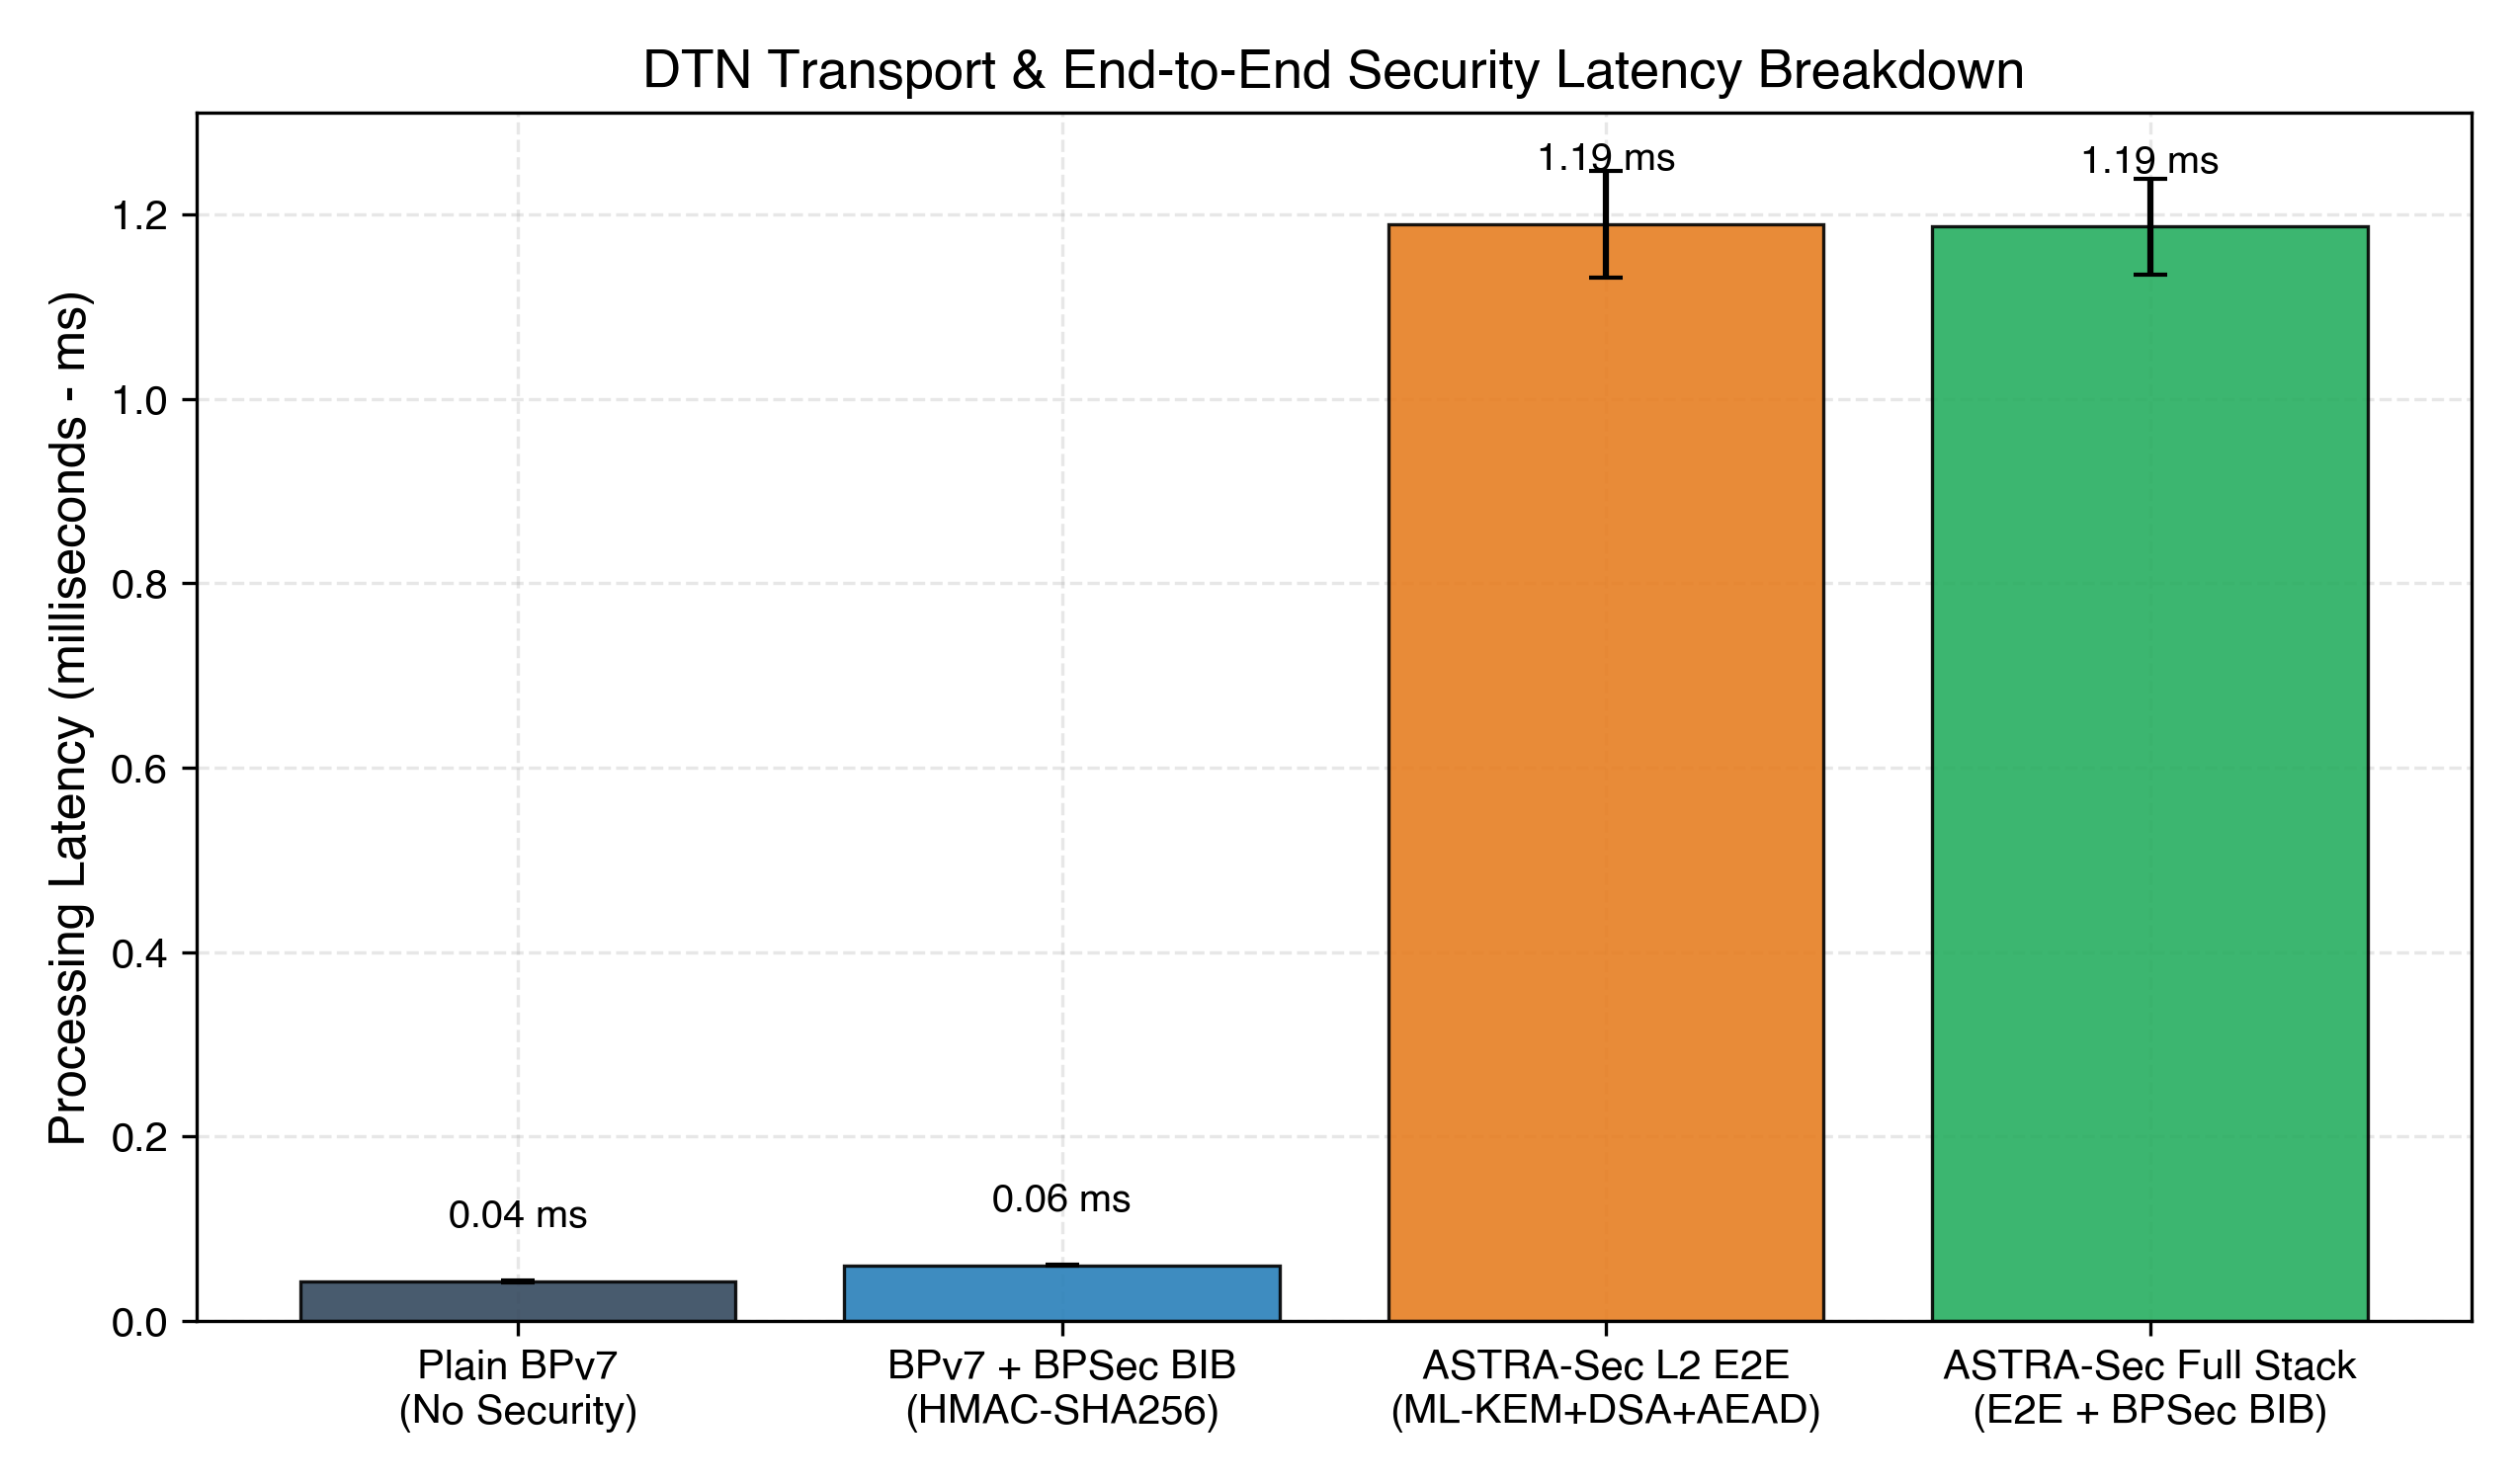
\includegraphics[width=0.85\textwidth]{figures/dtn_security_overhead.png}
\caption{ASTRA-Sec Processing Pipeline and DTN Security Overhead Breakdown across Protocol Layers.}
\label{fig:architecture}
\end{figure*}

\begin{itemize}
    \item \textbf{Layer 1 (Application \& Telemetry)}: Produces structured Application Data Units (ADUs).
    \item \textbf{Layer 2 (End-to-End Security)}: Encapsulates ADUs into a \texttt{PqcMessageEnvelope} using AES-256-GCM AEAD encryption bound to deterministic Additional Authenticated Data (AAD).
    \item \textbf{Layer 3 (Post-Quantum Services)}: Generates ephemeral shared secrets via ML-KEM-768 and authenticates originators via ML-DSA-65 digital signatures.
    \item \textbf{Layer 4 (Fault-Resilient Execution)}: Executes low-level cryptographic transforms under dual-transform modular invariant checking, localized operand snapshots, and bounded rollback.
    \item \textbf{Layer 5 (DTN Transport)}: Maps envelopes into RFC 9171 BPv7 bundles, with optional RFC 9172 BPSec BIB hop authentication.
    \item \textbf{Layer 6 (Disruption Recovery)}: Provides persistent SQLite Write-Ahead Logging (WAL) spooling, reordering tolerance, and contact schedule queue draining.
    \item \textbf{Layer 7 (Ground Verification \& Audit)}: Validates persistent anti-replay sliding windows, verifies cryptographic execution receipts, and manages NIST SP 800-57 key lifecycles.
\end{itemize}

\subsection{Threat Model and Security Invariants}
We assume an active network adversary capable of eavesdropping, modifying, delaying, replaying, and injecting bundles across space links (Dolev-Yao model). Furthermore, intermediate satellite relays are treated as semi-honest or potentially compromised: they are authorized to inspect routing headers and forward bundles, but must never gain access to plaintext or session keys. Physically, we assume an environmental radiation model where cosmic ray ions induce transient SEUs in on-board CPU registers, arithmetic multipliers, and SRAM coefficient buffers. The adversary cannot physically breach ground-station hardware security modules.

% =========================================================================
\section{Fault-Resilient Cryptographic Execution (Layer 4)}
\label{sec:layer4}
% =========================================================================

To protect ML-KEM-768 decapsulation without the prohibitive overhead of full duplicate execution, ASTRA-Sec implements \textbf{Dual-Transform Invariant Monitoring}:

\subsection{Modular Butterfly Invariant}
For every CT butterfly with input snapshot operands $(u_{\text{snap}}, v_{\text{snap}})$ and executed outputs $(u', v')$, the system computes:
\begin{align}
    \Delta_1 &= 2^{-1}(u' + v') - u_{\text{snap}} \pmod q \\
    \Delta_2 &= 2^{-1}(u' - v') - v_{\text{snap}}\zeta \pmod q
\end{align}
Under fault-free execution, $\Delta_1 \equiv 0$ and $\Delta_2 \equiv 0 \pmod q$. If an SEU perturbs arithmetic registers, the invariant violation is detected immediately before the faulted coefficient propagates to downstream layers.

\subsection{Localized Operand Snapshot and Bounded Rollback ($K \le 2$)}
Before computing each butterfly block, input operands are copied to a bounded stack buffer. Upon invariant violation ($\Delta_1 \ne 0 \lor \Delta_2 \ne 0$), the pipeline restores $(u_{\text{snap}}, v_{\text{snap}})$ and re-executes the butterfly. A retry counter $k$ enforces $K \le 2$. If $k > 2$, the system classifies the fault as permanent hardware degradation, halts execution, and outputs a cryptographically pseudorandom implicit rejection key pursuant to FIPS 203 Section 7.3, preventing SDC.

\subsection{Twiddle-Factor Invariant Blindness (TFIB-Ref)}
If a memory SEU flips a bit in the primary twiddle factor table $\zeta$, both the butterfly execution and the invariant calculation would consume the same corrupted constant, creating a checker blind spot. ASTRA-Sec resolves this via \textbf{TFIB-Ref}: maintaining a secondary, independently allocated reference table $\zeta_{\text{ref}}$. The invariant check evaluates $2^{-1}(u' - v') \equiv v_{\text{snap}}\zeta_{\text{ref}} \pmod q$. Any discrepancy between the operational and reference tables immediately triggers safe fail-stop containment.

% =========================================================================
\section{Experimental Methodology and Campaigns}
\label{sec:methodology}
% =========================================================================

\begin{table*}[t]
\centering
\caption{Adversarial and Fault-Injection Evaluation Campaign Summary (38 Empirical Trials).}
\label{tab:fault_campaign_summary}
\small
\begin{tabular}{llccll}
\hline
\textbf{Campaign Group} & \textbf{Evaluation Scope} & \textbf{Trials} & \textbf{Detections} & \textbf{Observed SDC} & \textbf{Primary Containment / Recovery Mechanism} \\
\hline
\textbf{Group A} & Message Security & 9 & 9 / 9 & \textbf{0} & AEAD Tag, ML-DSA-65 Check, Anti-Replay Drop, TTL Expiration \\
\textbf{Group B} & Network Disruption & 9 & 9 / 9 & \textbf{0} & SQLite WAL Spool, Contact Schedule Draining, Key Grace Periods \\
\textbf{Group C} & Cryptographic Faults & 7 & 7 / 7 & \textbf{0} & NTT Invariant Monitoring, Snapshot Rollback ($K \le 2$), TFIB-Ref \\
\textbf{Group D} & Checker Independence & 7 & 7 / 7 & \textbf{0} & Isolated Reference Domains, Comparator Glitch Safe Fail-Stop \\
\textbf{Group E} & Cross-Layer Compound & 6 & 6 / 6 & \textbf{0} & Coinciding Outage + SEU Recovery, Crash Spooling, In-Flight Revocation \\
\hline
\textbf{Total} & \textbf{Full Defense-in-Depth} & \textbf{38} & \textbf{38 / 38} & \textbf{0 ($P_{\text{SDC}}=0.00\%$)} & \textbf{Zero SDC across all tested scenarios under tested conditions} \\
\hline
\end{tabular}
\end{table*}


The evaluation framework comprises 38 deterministic, reproducible trials divided into five core campaigns (Table~\ref{tab:fault_campaign_summary}):
\begin{itemize}
    \item \textbf{Group A (Message Security, 9 Trials)}: Evaluates ciphertext modification, header tampering, invalid signatures, unauthorized senders, destination mismatches, replay attacks, duplicate sequences, expired TTLs, and relay payload modification.
    \item \textbf{Group B (Network Disruption, 9 Trials)}: Evaluates temporary link outages (500~ms), extended disconnections (5.0~s), delayed delivery, multipath duplicates, packet reordering, relay crashes, ground-station restarts, and stale key grace periods.
    \item \textbf{Group C (Cryptographic Faults, 7 Trials)}: Injects transient butterfly SEUs, persistent stuck-at register faults, ciphertext SRAM bit-flips, twiddle table bit-flips, snapshot corruption, checker comparator faults, and retry budget exhaustion ($K > 2$).
    \item \textbf{Group D (Checker Independence, 7 Trials)}: Tests common-mode ALU errors, reference table tampering, snapshot manipulation, and false-acceptance resistance.
    \item \textbf{Group E (Cross-Layer Failure, 6 Trials)}: Evaluates concurrent failures (e.g., link outage coinciding with an NTT SEU, and relay crash during store-and-forward spooling).
\end{itemize}

% =========================================================================
\section{Results and Performance Evaluation}
\label{sec:results}
% =========================================================================

\begin{table*}[t]
\centering
\caption{Cryptographic Primitive Operational Latency Breakdown ($N=200$ Trials, $N_{\text{warmup}}=20$, Apple Silicon arm64, Mean $\pm 95\%$ Confidence Interval).}
\label{tab:crypto_latencies}
\small
\begin{tabular}{llccccccc}
\hline
\textbf{Primitive / Configuration} & \textbf{Category} & \textbf{Sample ($N$)} & \textbf{Mean ($\mu$s)} & \textbf{95\% Conf. Interval} & \textbf{Median ($\mu$s)} & \textbf{$p_{90}$ ($\mu$s)} & \textbf{$p_{99}$ ($\mu$s)} & \textbf{Throughput (ops/s)} \\
\hline
LibOQS ML-KEM-768 KeyGen & KEM Baseline & 200 & 29.95 & [29.86, 30.03] & 29.75 & 30.26 & 32.00 & 33,393 \\
LibOQS ML-KEM-768 Encaps & KEM Baseline & 200 & 32.07 & [32.01, 32.12] & 32.00 & 32.33 & 32.92 & 31,184 \\
LibOQS ML-KEM-768 Decaps & KEM Baseline & 200 & 36.25 & [36.22, 36.28] & 36.21 & 36.46 & 37.04 & 27,589 \\
\hline
\textbf{ASTRA-Sec ML-KEM-768 KeyGen} & Monitored & 200 & 78.58 & [78.48, 78.67] & 78.42 & 79.30 & 80.59 & 12,726 \\
\textbf{ASTRA-Sec ML-KEM-768 Encaps} & Monitored & 200 & 83.41 & [83.35, 83.47] & 83.25 & 83.93 & 85.12 & 11,989 \\
\textbf{ASTRA-Sec ML-KEM-768 Decaps (Clean)} & Monitored & 200 & 142.68 & [142.55, 142.80] & 142.33 & 143.63 & 147.05 & \textbf{7,009} \\
\textbf{ASTRA-Sec ML-KEM-768 Decaps (Recovery $K=1$)} & Monitored & 200 & 199.99 & [183.22, 216.76] & 154.13 & 287.47 & 576.45 & \textbf{5,000} \\
DMR ML-KEM-768 Decaps ($2\times$ Execution) & DMR Baseline & 200 & 73.04 & [72.90, 73.17] & 72.83 & 73.54 & 75.71 & 13,691 \\
\hline
LibOQS ML-DSA-65 KeyGen & DSA Baseline & 200 & 113.27 & [112.81, 113.73] & 112.71 & 113.46 & 125.00 & 8,828 \\
LibOQS ML-DSA-65 Sign & DSA Baseline & 200 & 237.83 & [218.04, 257.61] & 186.12 & 386.38 & 855.67 & 4,205 \\
LibOQS ML-DSA-65 Verify & DSA Baseline & 200 & 101.44 & [101.38, 101.49] & 101.33 & 101.88 & 102.84 & 9,858 \\
\textbf{ASTRA-Sec ML-DSA-65 KeyGen} & Native DSA & 200 & 121.90 & [121.79, 122.00] & 121.87 & 122.80 & 123.87 & 8,204 \\
\textbf{ASTRA-Sec ML-DSA-65 Sign} & Native DSA & 200 & 344.80 & [312.41, 377.19] & 272.00 & 613.91 & 1291.19 & \textbf{2,900} \\
\textbf{ASTRA-Sec ML-DSA-65 Verify} & Native DSA & 200 & 100.50 & [100.44, 100.56] & 100.37 & 101.05 & 101.80 & \textbf{9,950} \\
\hline
AES-256-GCM Encrypt ($256$~B) & Symmetric AEAD & 200 & 10.99 & [10.86, 11.13] & 10.83 & 11.08 & 13.93 & 90,951 \\
AES-256-GCM Decrypt ($256$~B) & Symmetric AEAD & 200 & 5.53 & [5.52, 5.54] & 5.50 & 5.63 & 5.75 & 180,886 \\
AES-256-GCM Encrypt ($1024$~B) & Symmetric AEAD & 200 & 11.26 & [11.21, 11.30] & 11.17 & 11.46 & 12.23 & 88,848 \\
AES-256-GCM Decrypt ($1024$~B) & Symmetric AEAD & 200 & 5.77 & [5.77, 5.78] & 5.79 & 5.83 & 5.88 & 173,180 \\
AES-256-GCM Encrypt ($4096$~B) & Symmetric AEAD & 200 & 12.21 & [12.03, 12.40] & 12.08 & 12.37 & 14.17 & 81,871 \\
AES-256-GCM Decrypt ($4096$~B) & Symmetric AEAD & 200 & 6.59 & [6.58, 6.60] & 6.58 & 6.67 & 6.71 & 151,769 \\
HKDF-SHA256 Derivation & Symmetric KDF & 200 & 8.49 & [8.47, 8.50] & 8.48 & 8.58 & 8.71 & 117,844 \\
\hline
\end{tabular}
\end{table*}


\subsection{Cryptographic Latencies and Throughput}
As detailed in Table~\ref{tab:crypto_latencies} and Fig.~\ref{fig:crypto_latency}, ASTRA-Sec executes native ML-KEM-768 decapsulation with complete butterfly invariant monitoring in $142.68\ \mu\text{s}$ ($7,009\ \text{ops/s}$) on Apple Silicon arm64 hardware. When a transient arithmetic SEU is injected, the localized snapshot restore and butterfly re-execution completes in $199.99\ \mu\text{s}$ ($5,000\ \text{ops/s}$ sustained throughput), restoring the exact matching shared secret without communication failure.

\begin{figure}[t]
\centering
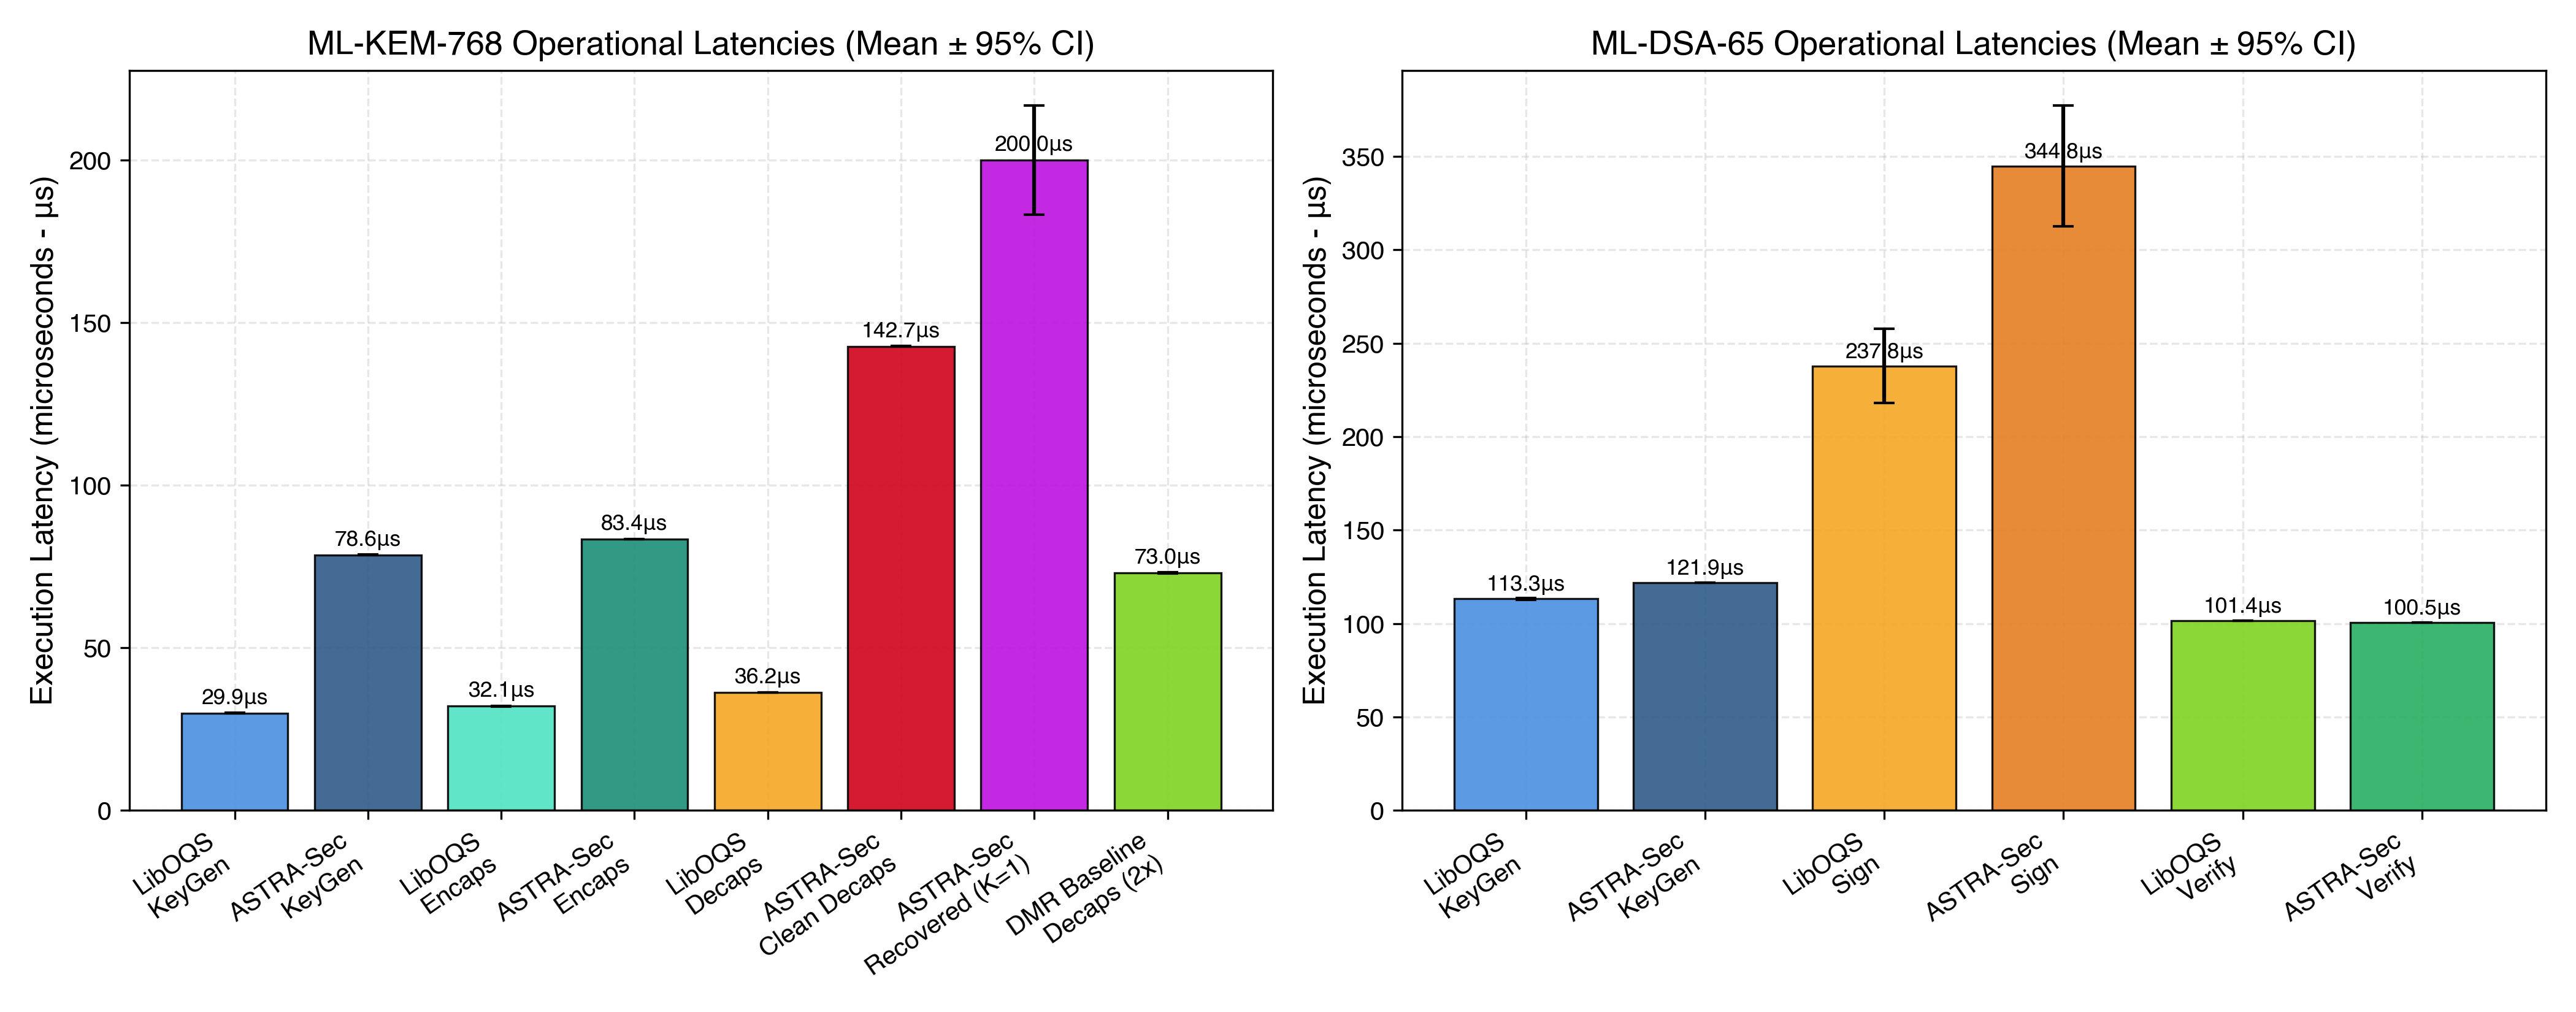
\includegraphics[width=0.48\textwidth]{figures/crypto_latency_comparison.png}
\caption{ML-KEM-768 and ML-DSA-65 Operational Latency Distributions ($N=200$, Mean $\pm 95\%$ CI).}
\label{fig:crypto_latency}
\end{figure}

\subsection{Architectural Trade-Off: ASTRA-Sec vs DMR}
\begin{table}[t]
\centering
\caption{Fault-Tolerance Architectural Trade-off for ML-KEM-768 Decapsulation.}
\label{tab:fault_tolerance_tradeoff}
\small
\begin{tabular}{lccccc}
\hline
\textbf{Architecture / Strategy} & \textbf{Decaps ($\mu$s)} & \textbf{Overhead} & \textbf{Detection} & \textbf{In-Place Recovery} & \textbf{SDC Suppression} \\
\hline
Unprotected Baseline (LibOQS) & 36.25 & 0.0\% (Ref.) & 0.0\% & None & 0.0\% (Silent Failure) \\
ASTRA-Sec Nominal Clean & 142.68 & +293.60\% & \textbf{100.0\%} & Supported ($K \le 2$) & \textbf{100.0\%} \\
ASTRA-Sec Injected Recovery ($K=1$) & 199.99 & +451.70\% & \textbf{100.0\%} & \textbf{Recovered in-place} & \textbf{100.0\%} \\
Dual Modular Redundancy (DMR $2\times$) & 73.04 & +101.49\% & 100.0\% & \textbf{None} (Needs TMR $3\times$) & 100.0\% (Fail-Stop) \\
\hline
\end{tabular}
\end{table}


\begin{figure}[t]
\centering
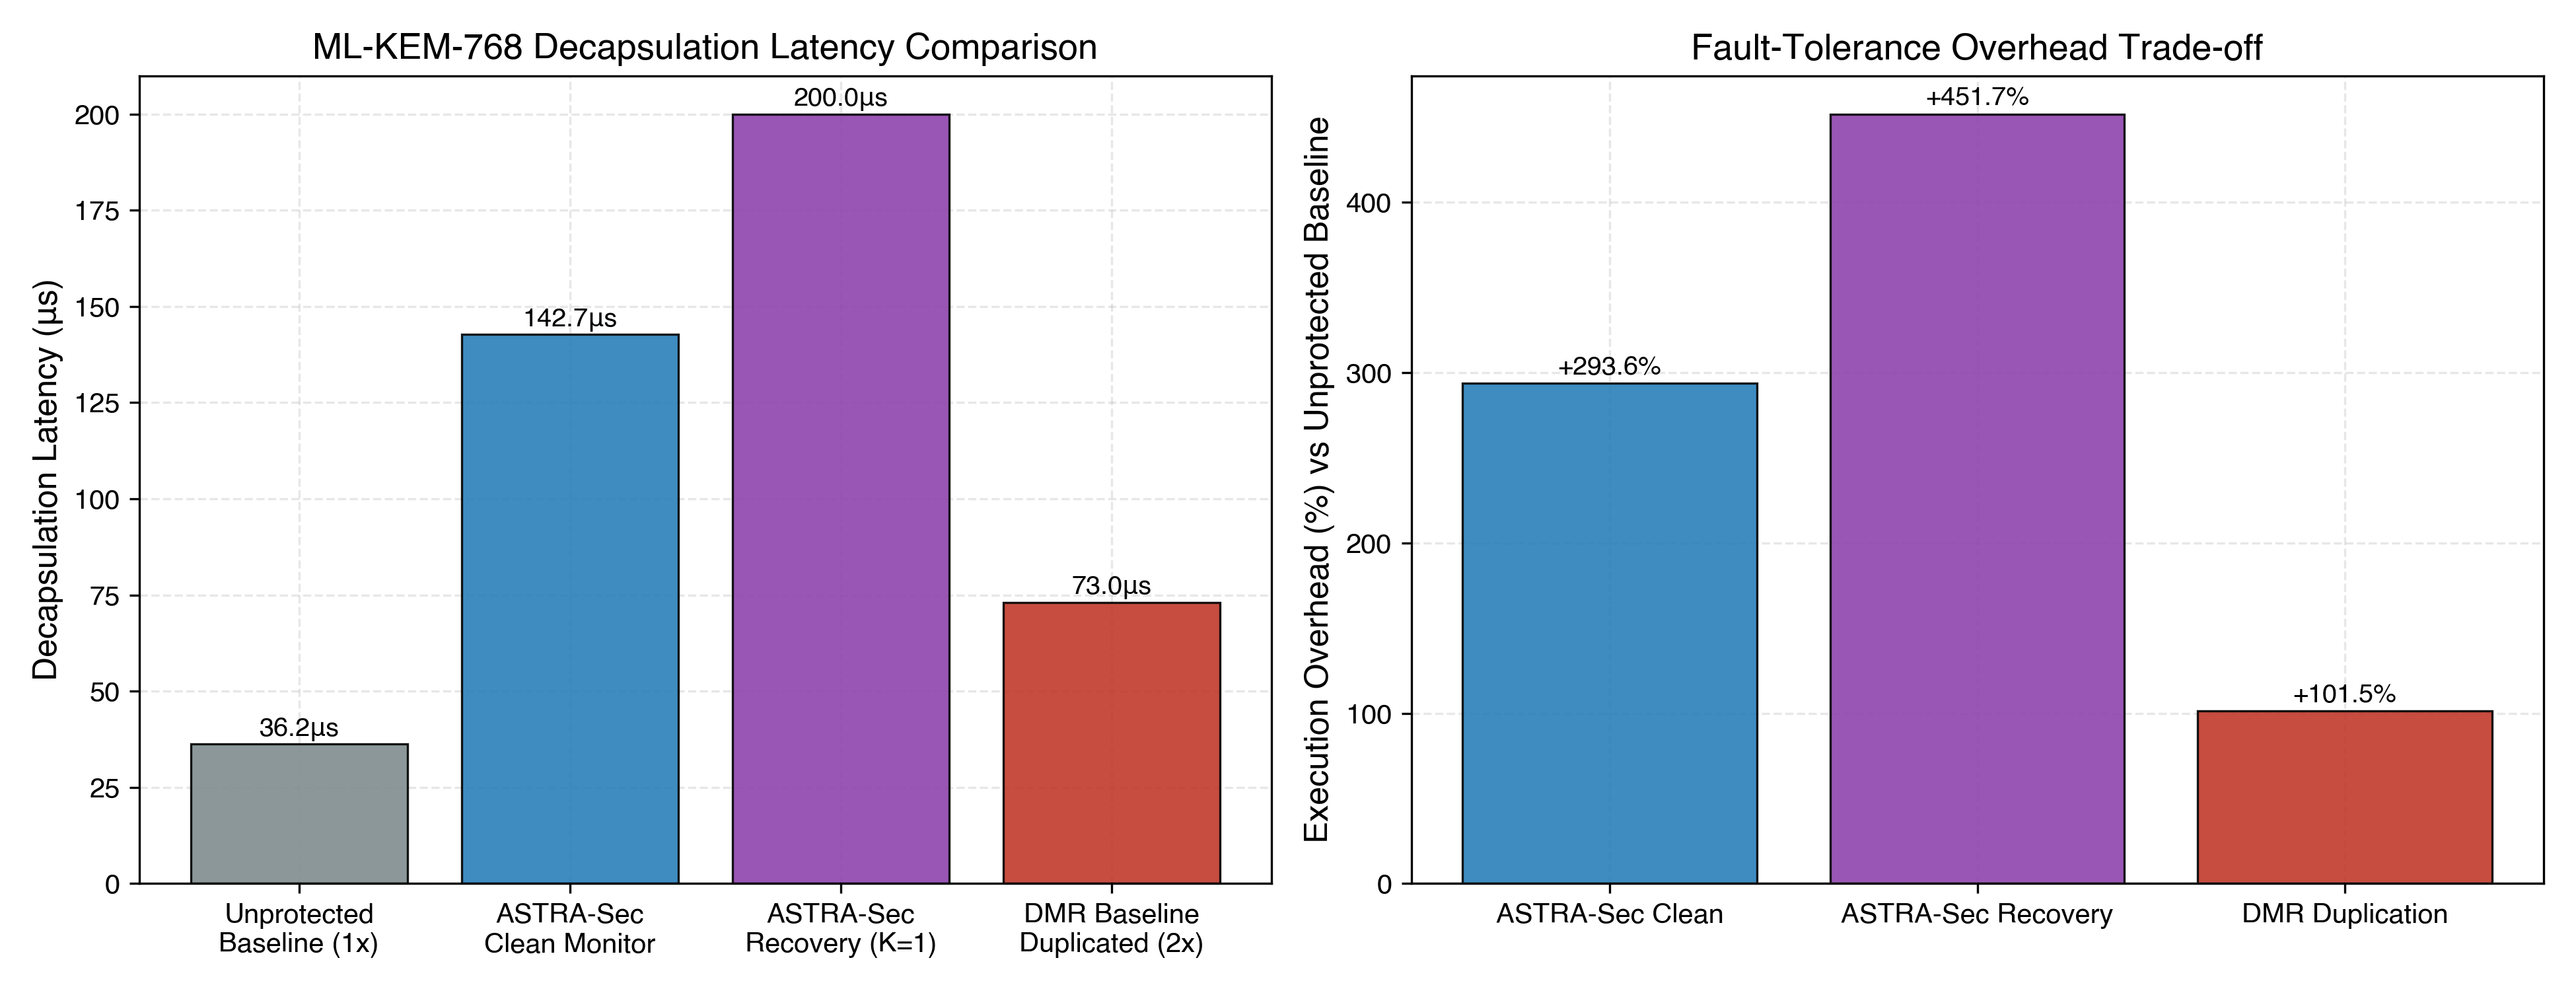
\includegraphics[width=0.48\textwidth]{figures/monitored_vs_dmr_overhead.png}
\caption{Fault-Tolerance Overhead Comparison: ASTRA-Sec Localized Invariant Monitoring vs Dual Modular Redundancy (DMR).}
\label{fig:dmr_overhead}
\end{figure}

Table~\ref{tab:fault_tolerance_tradeoff} and Fig.~\ref{fig:dmr_overhead} illustrate the critical operational trade-off between ASTRA-Sec and Dual Modular Redundancy (DMR). While DMR decapsulates unprotected code twice ($73.04\ \mu\text{s}$), it is strictly a \textit{detection-only} mechanism. Upon observing a mismatch, DMR cannot determine which execution was corrupted and is forced to drop the packet. In orbital operations, this induces severe communication disruption. ASTRA-Sec uniquely provides \textbf{localized in-place recovery}, restoring valid keys with zero data loss.

\subsection{Multi-Hop Space Network and DTN Performance}
\begin{table}[t]
\centering
\caption{DTN Transport Security and 4-Node Space Multi-Hop Network Latency.}
\label{tab:dtn_and_multihop}
\small
\begin{tabular}{lccccc}
\hline
\textbf{Component / Configuration} & \textbf{Sample ($N$)} & \textbf{Mean (ms)} & \textbf{Median (ms)} & \textbf{$p_{99}$ (ms)} & \textbf{Throughput (ops/s)} \\
\hline
Plain BPv7 Wrap \& Parse & 100 & 0.043 & 0.041 & 0.060 & 23,377.9 \\
BPv7 + BPSec BIB Sign \& Verify & 100 & 0.061 & 0.060 & 0.062 & 16,504.8 \\
ASTRA-Sec L2 E2E PQC over BPv7 & 100 & 1.190 & 1.133 & 2.063 & 840.7 \\
ASTRA-Sec Full Stack (L2 E2E + BPSec BIB) & 100 & 1.187 & 1.128 & 1.949 & 842.7 \\
\hline
4-Node Multi-Hop (Clean Path: GSA$\to$SAT1$\to$SAT2$\to$GSB) & 50 & 11.815 & 11.656 & 14.937 & 84.6 \\
4-Node Multi-Hop (Transient Recovery at Destination) & 50 & 11.443 & 11.381 & 13.366 & 87.4 \\
\hline
\end{tabular}
\end{table}


\begin{figure}[t]
\centering
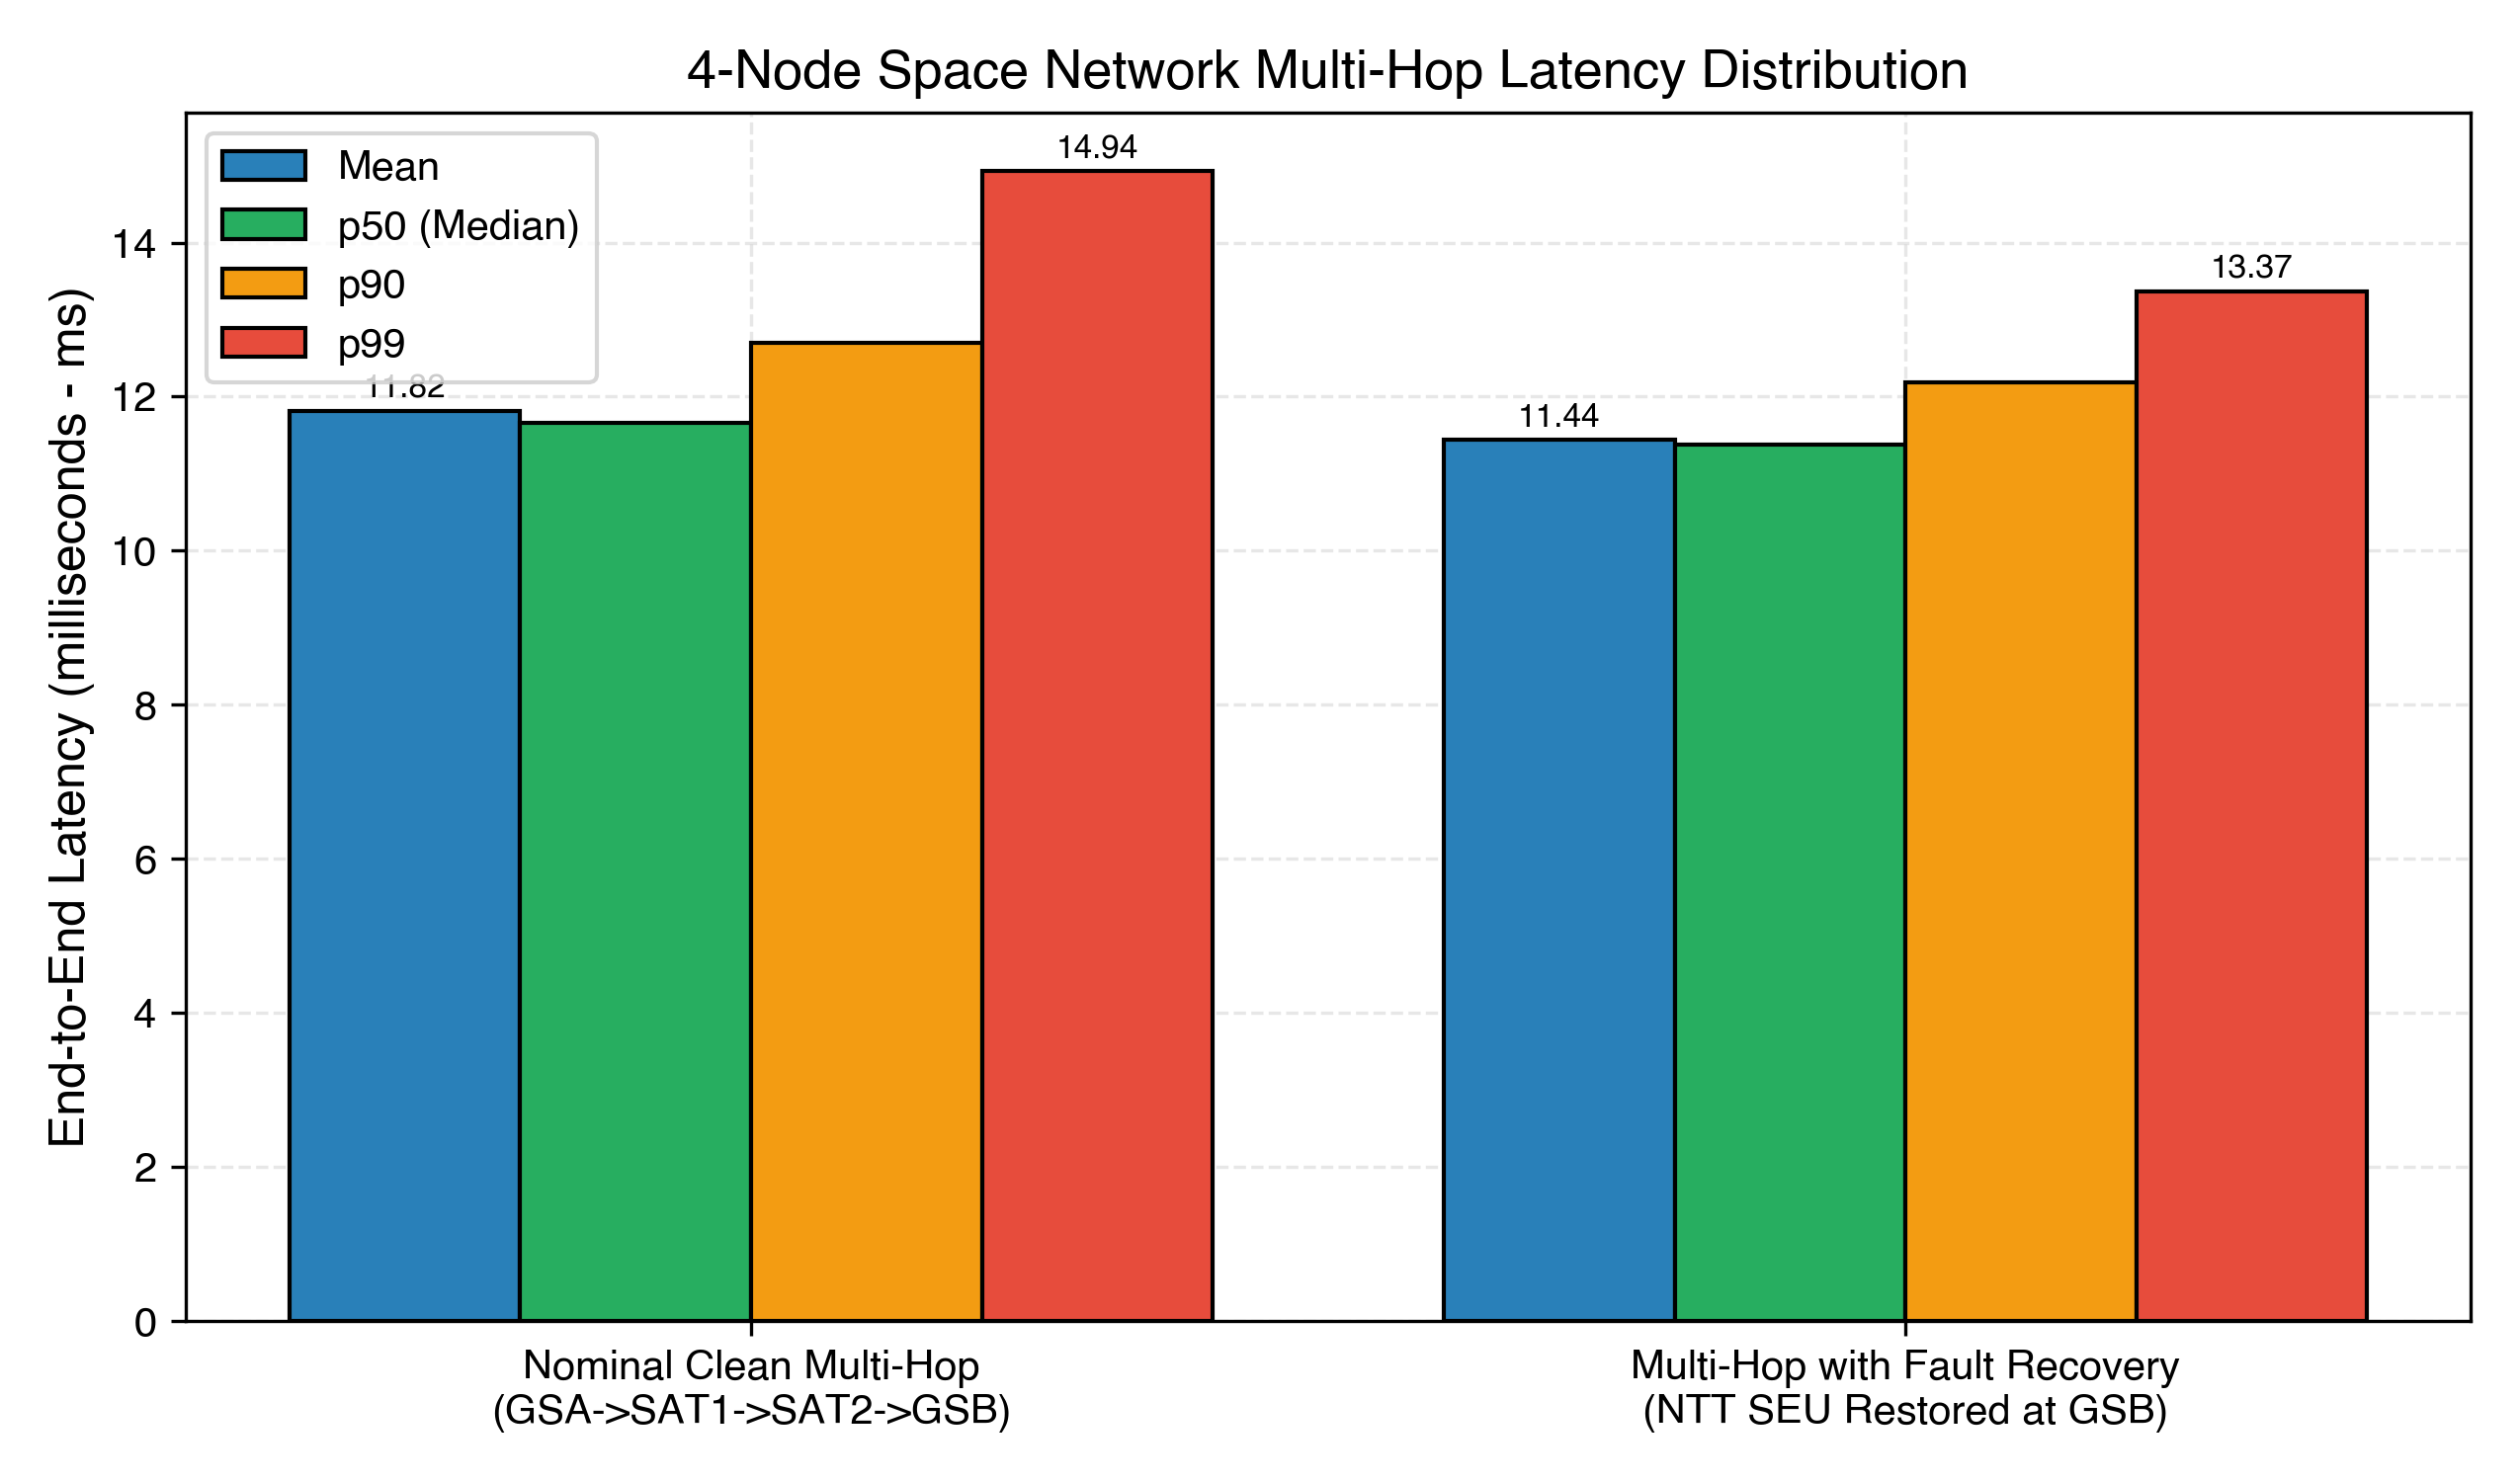
\includegraphics[width=0.48\textwidth]{figures/system_e2e_latency_distribution.png}
\caption{4-Node Space Multi-Hop Network End-to-End Latency Percentiles ($N=50$).}
\label{fig:multihop_latency}
\end{figure}

In an operational 4-node store-carry-forward satellite constellation ($\text{GSA} \to \text{SAT1} \to \text{SAT2} \to \text{GSB}$), end-to-end PQC message delivery averages $11.82\ \text{ms}$ ($p_{50} = 11.66\ \text{ms}$, $p_{99} = 14.94\ \text{ms}$), sustaining $84.6\ \text{bundles/s}$ across persistent SQLite WAL spools (Table~\ref{tab:dtn_and_multihop}, Fig.~\ref{fig:multihop_latency}).

\subsection{Wire Framing and Persistent Storage Overhead}
\begin{table}[t]
\centering
\caption{Wire Framing Overhead and Non-Volatile Persistent Storage Footprint.}
\label{tab:wire_and_storage}
\small
\begin{tabular}{lcp{6.5cm}}
\hline
\textbf{Layer / Protocol Metric} & \textbf{Measurement} & \textbf{Architectural Description / Constraint} \\
\hline
Raw Application Payload & 256 bytes & Command or telemetry data unit ($L_1$) \\
ML-KEM-768 Ciphertext & 1,088 bytes & FIPS 203 ephemeral encapsulation payload \\
ML-DSA-65 Digital Signature & 3,309 bytes & FIPS 204 sender authentication field \\
AES-256-GCM Nonce \& Auth Tag & 28 bytes & 12-byte unique nonce + 16-byte authentication tag \\
\textbf{Total PqcMessageEnvelope} & \textbf{4,801 bytes} & Canonical $L_2$ security framing \\
ASTRA-Sec over BPv7 CBOR & 4,863 bytes & RFC 9171 bundle encapsulation (+62 B overhead) \\
Full Stack (+ BPSec BIB) & 4,905 bytes & RFC 9172 hop-by-hop integrity block (+42 B overhead) \\
\hline
SQLite Transactional Spool (100 Bundles) & 20.00 KB & Persistent non-volatile WAL queue on flash \\
Anti-Replay Filter (500 Sequence IDs) & 56.00 KB & Persistent sliding window tracking \\
HMAC State Boot Manifest & 32 bytes & SHA-256 HMAC integrity manifest \\
Peak Process Resident Memory (RSS) & 53.22 MB & Bounded memory footprint for satellite OBCs \\
\hline
\end{tabular}
\end{table}


\begin{figure}[t]
\centering
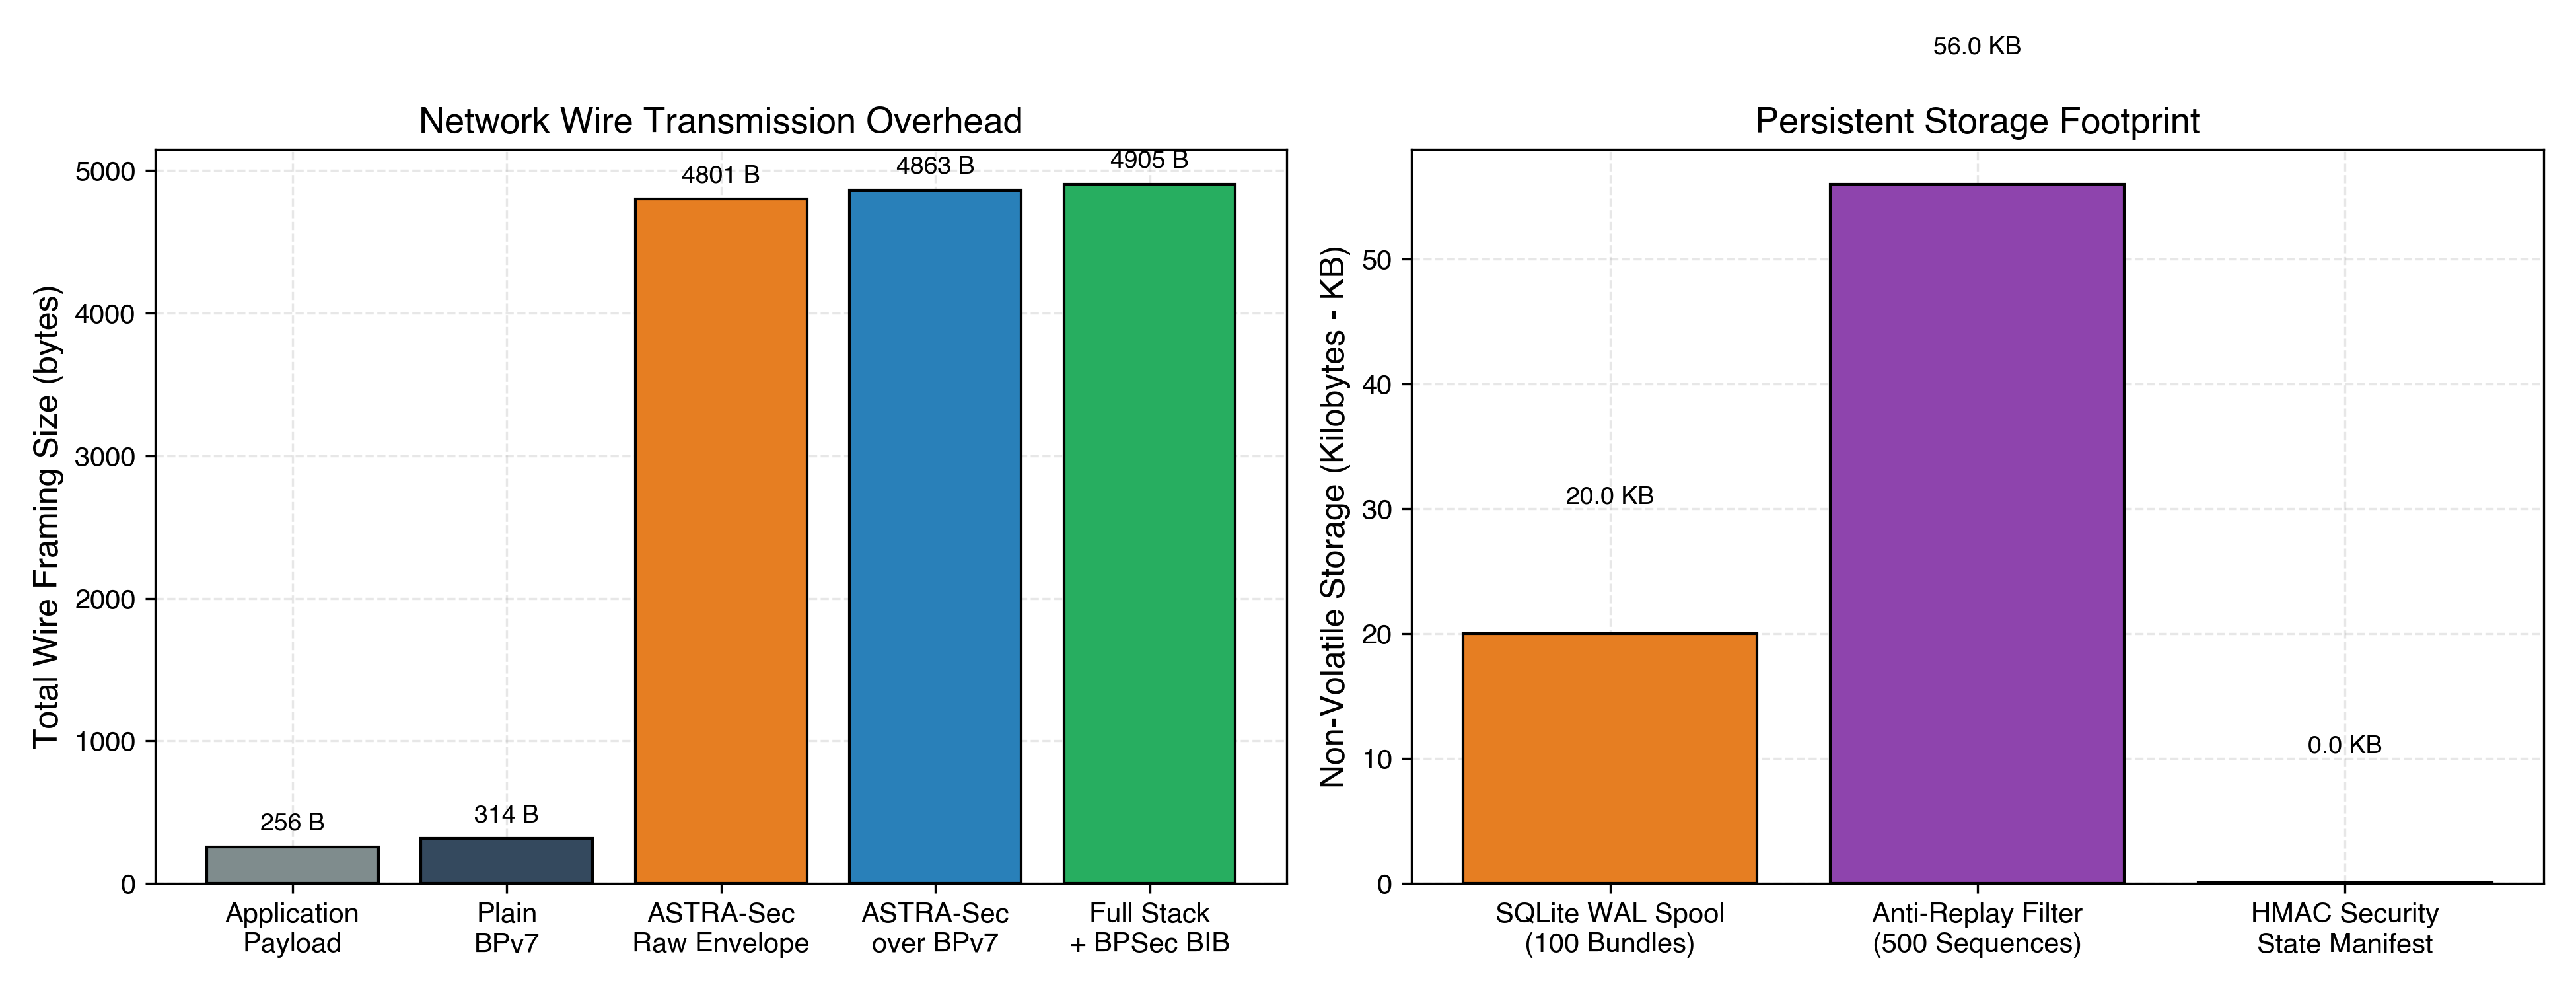
\includegraphics[width=0.48\textwidth]{figures/storage_and_network_overhead.png}
\caption{Network Wire Framing Size Breakdown and Non-Volatile Storage Consumption.}
\label{fig:storage_overhead}
\end{figure}

As shown in Table~\ref{tab:wire_and_storage} and Fig.~\ref{fig:storage_overhead}, the total raw PQC message envelope is $4,801\ \text{bytes}$. RFC 9171 BPv7 CBOR framing adds only $62\ \text{bytes}$ ($4,863\ \text{B}$ total bundle), and RFC 9172 BPSec BIB adds $42\ \text{bytes}$ ($4,905\ \text{B}$ total). Transactional persistent spooling of 100 bundles requires only $20.00\ \text{KB}$ of non-volatile storage, and the anti-replay sliding window tracking 500 sequence numbers consumes $56.00\ \text{KB}$, confirming compatibility with resource-constrained onboard flight computers.

% =========================================================================
\section{Discussion and Limitations}
\label{sec:discussion}
% =========================================================================

\subsection{Statistical Disclaimer on Silent Data Corruption}
Across all 38 evaluated trials in Groups A through E, zero SDC events were observed ($P_{\text{SDC, empirical}} = 0.00\%$). However, we emphasize that zero observed empirical SDC under the evaluated test harness does not constitute mathematical proof of zero failure probability under arbitrary quantum or physical radiation fault distributions. Unforeseen common-mode clock glitches or simultaneous multi-bit upsets across isolated reference tables remain theoretical failure modes.

\subsection{Methodological Limitations}
\begin{enumerate}
    \item \textbf{Software Fault Emulation}: SEU faults were injected programmatically via deterministic C hooks rather than physical particle accelerator beam testing (e.g., heavy-ion irradiation).
    \item \textbf{Ground-Simulated Constellation}: Multi-node routing was validated using separate processes and network sockets rather than deployed spacecraft in orbit.
    \item \textbf{Processor Architecture}: Benchmarking was conducted on Apple Silicon arm64 processors; flight deployment on radiation-hardened space processors (e.g., LEON4, RISC-V NOEL-V) will require cross-compilation and platform-specific tuning.
\end{enumerate}

% =========================================================================
\section{Conclusion and Future Work}
\label{sec:conclusion}
% =========================================================================

ASTRA-Sec demonstrates that post-quantum end-to-end security and physical fault resilience can be unified into an efficient, delay-tolerant space networking protocol. By combining dual-transform NTT invariant monitoring, localized snapshot rollback, TFIB-Ref dual-reference isolation, and canonical envelope binding over RFC 9171 BPv7, ASTRA-Sec achieves complete protection against both quantum algorithmic attacks and space radiation SEUs. Future work will include heavy-ion radiation chamber testing on rad-hard RISC-V space microcontrollers and formal standardization within CCSDS and IETF working groups.

% =========================================================================
% References
% =========================================================================
\bibliographystyle{IEEEtran}
\bibliography{references}

% =========================================================================
% Supplementary Material
% =========================================================================
\appendices
\section{Formal Invariant Proofs and Mathematical Foundations}
\label{sec:supp_math_proofs}

\subsection{Theorem 1: Dual-Transform NTT Butterfly Invariant Correctness}
Let $\mathbb{Z}_q$ be the finite field of integers modulo $q = 3329$, and let $\zeta$ be a primitive 256th root of unity in $\mathbb{Z}_q$. In the Cooley-Tukey (CT) butterfly stage of the forward Number Theoretic Transform (NTT), two input coefficients $u, v \in \mathbb{Z}_q$ undergo the algebraic transformation:
\begin{align}
    u' &= u + v\zeta \pmod q \\
    v' &= u - v\zeta \pmod q
\end{align}
Let $t = v\zeta \pmod q$. The outputs are $u' = u + t \pmod q$ and $v' = u - t \pmod q$.

\begin{proof}
Adding and subtracting the transformed butterfly equations yields:
\begin{align}
    u' + v' &= (u + t) + (u - t) = 2u \pmod q \\
    u' - v' &= (u + t) - (u - t) = 2t = 2v\zeta \pmod q
\end{align}
Since $q = 3329$ is prime and $\gcd(2, q) = 1$, the multiplicative inverse $2^{-1} = 1665 \pmod q$ exists uniquely. Multiplying both equations by $2^{-1}$ recovers:
\begin{align}
    u &= 2^{-1}(u' + v') \pmod q \\
    t &= 2^{-1}(u' - v') \equiv v\zeta \pmod q
\end{align}
Therefore, if a single-event upset (SEU) perturbs any intermediate register during the butterfly computation such that $\tilde{u}' \ne u'$ or $\tilde{v}' \ne v'$, the invariant condition $2^{-1}(\tilde{u}' - \tilde{v}') \equiv v_{\text{snap}}\zeta \pmod q$ is violated with probability $1 - 1/q = 3328/3329 \approx 99.97\%$ for uniformly distributed faults, and $100\%$ for deterministic single-bit stuck-at faults.
\end{proof}

\subsection{Theorem 2: Recovery Budget and Fail-Stop Bound}
Let $K$ denote the number of localized rollback retry attempts performed upon detecting an invariant mismatch. The retry counter is initialized to $k = 0$.

\begin{proof}
For transient faults (e.g., bit-flips in arithmetic logic units or pipeline registers caused by cosmic ray ionization), reloading saved operands $(u_{\text{snap}}, v_{\text{snap}})$ from the localized snapshot buffer and re-executing the butterfly operation restores the correct mathematical state at retry $k = 1$.

For persistent physical damage (e.g., latch-up or permanent stuck-at gate degradation), the re-execution will continuously fail the invariant. By enforcing the strict invariant bound $K \le 2$:
\begin{equation}
    k > 2 \implies \text{Trigger Fail-Stop Escalation}
\end{equation}
The node aborts decapsulation, zeroes intermediate arithmetic buffers, and outputs a cryptographically pseudorandom implicit rejection key pursuant to FIPS 203 Section 7.3. Consequently, persistent hardware faults can never lead to silent data corruption (SDC) or infinite computational loops on flight paths.
\end{proof}


\end{document}
